We apply a data-driven method to estimate the jet veto 
efficiency and its systematic uncertainties in data. 
In this method, the jet veto efficiency on $\WW$ events in data $\epsilon_{\WW}$
is estimated to be the value obtained from simulation multiplied by a data to simulation
scale factor from \dyll~events such that,

\begin{center}
$\epsilon_{WW} = \epsilon_{WW}^{MC} (\frac{\epsilon_{Z}^{data}}{\epsilon_{Z}^{MC}})$
\end{center}

The jet veto efficiency uncertainty of $WW$ can be factorized into 
the $Z$ efficiency uncertainty in data and $WW/Z$ efficiency ratio uncertainty in simulation. 
The former is statistically dominated, while theoretical uncertainties due to 
higher order corrections contribute most to the $WW/Z$ efficiency ratio uncertainties. 

The $\dyll$ jet veto efficiencies are measured in data and compared with the 
values obtained from Powheg and Madgraph simulations. 
Fig.~\ref{fig:zJetVetoEff} shows the dependence of the $\dyll$ 
jet veto efficiency on the jet $p_T$, comparing data and three different 
simulations. The results for three jet veto cuts 
are summarized in Tab.~\ref{tab:zeff_jec_results}. 
The data over simulation correction factor is found to be consistent with unity with the 
current jet veto thresold of 30 GeV. 

The theoretical uncertainties on the $WW/Z$ jet veto efficiency is evaluated by 
assessing the impact by the scale variations in both MCFM and MC@NLO. 
The uncertainty is quantified as the maximum change induced varying the 
renormalization and factorization scales independently. Details are given in Ref.~\cite{jetvetonote}. 
The relative systematic uncertainty is found to be 4.6\%. 

%%%%%%%%%%%%%%%%%%%%%5
\begin{table}[!htb]
\begin{center}
\begin{tabular}{|c|c|ccc|}
\hline
 samples &  all vtx bins & nVtx $<=$ 5 &  5 $<$ nVtx $<$ 10 & nVtx $>=$ 10 \\
\hline
\multicolumn{5}{|c|} {$ee$ Final State } \\ \hline
data & 0.83 $\pm$ 0.00 & 0.84 $\pm$ 0.00 & 0.83 $\pm$ 0.00 & 0.81 $\pm$ 0.00 \\
powheg MC & 0.83 $\pm$ 0.00 & 0.85 $\pm$ 0.00 & 0.83 $\pm$ 0.00 & 0.80 $\pm$ 0.00 \\
madgraph MC & 0.82 $\pm$ 0.00 & 0.84 $\pm$ 0.00 & 0.82 $\pm$ 0.00 & 0.79 $\pm$ 0.00 \\
\hline
data/powheg MC & 1.00 $\pm$ 0.00 & 0.99 $\pm$ 0.00 & 1.00 $\pm$ 0.00 & 1.01 $\pm$ 0.00 \\
data/madgraph MC & 1.01 $\pm$ 0.00 & 1.00 $\pm$ 0.00 & 1.01 $\pm$ 0.00 & 1.03 $\pm$ 0.00 \\
\hline
\multicolumn{5}{|c|} {$\mu\mu$ Final State } \\ \hline
data & 0.83 $\pm$ 0.00 & 0.85 $\pm$ 0.00 & 0.84 $\pm$ 0.00 & 0.82 $\pm$ 0.00 \\
powheg MC & 0.84 $\pm$ 0.00 & 0.85 $\pm$ 0.00 & 0.84 $\pm$ 0.00 & 0.81 $\pm$ 0.00 \\
madgraph MC & 0.82 $\pm$ 0.00 & 0.84 $\pm$ 0.00 & 0.83 $\pm$ 0.00 & 0.79 $\pm$ 0.00 \\
\hline
data/powheg MC & 1.00 $\pm$ 0.00 & 0.99 $\pm$ 0.00 & 0.99 $\pm$ 0.00 & 1.01 $\pm$ 0.00 \\
data/madgraph MC & 1.01 $\pm$ 0.00 & 1.01 $\pm$ 0.00 & 1.01 $\pm$ 0.00 & 1.03 $\pm$ 0.00 \\
\hline
\end{tabular}
\end{center}
\caption{
The jet veto efficiency and its data/simulation ratios on $Z$ events, 
using particle flow jets with the corrections described in Section~\ref{sec:sel_jets}. 
}
\label{tab:zeff_jec_results_ee}
\end{table}


%%%%%%%%%%%%%%%%%%%%%5
%%%%%%%%%%%%%%%%%%%%%%%%%%%%%%
\begin{figure}[htb]
  \begin{center}
   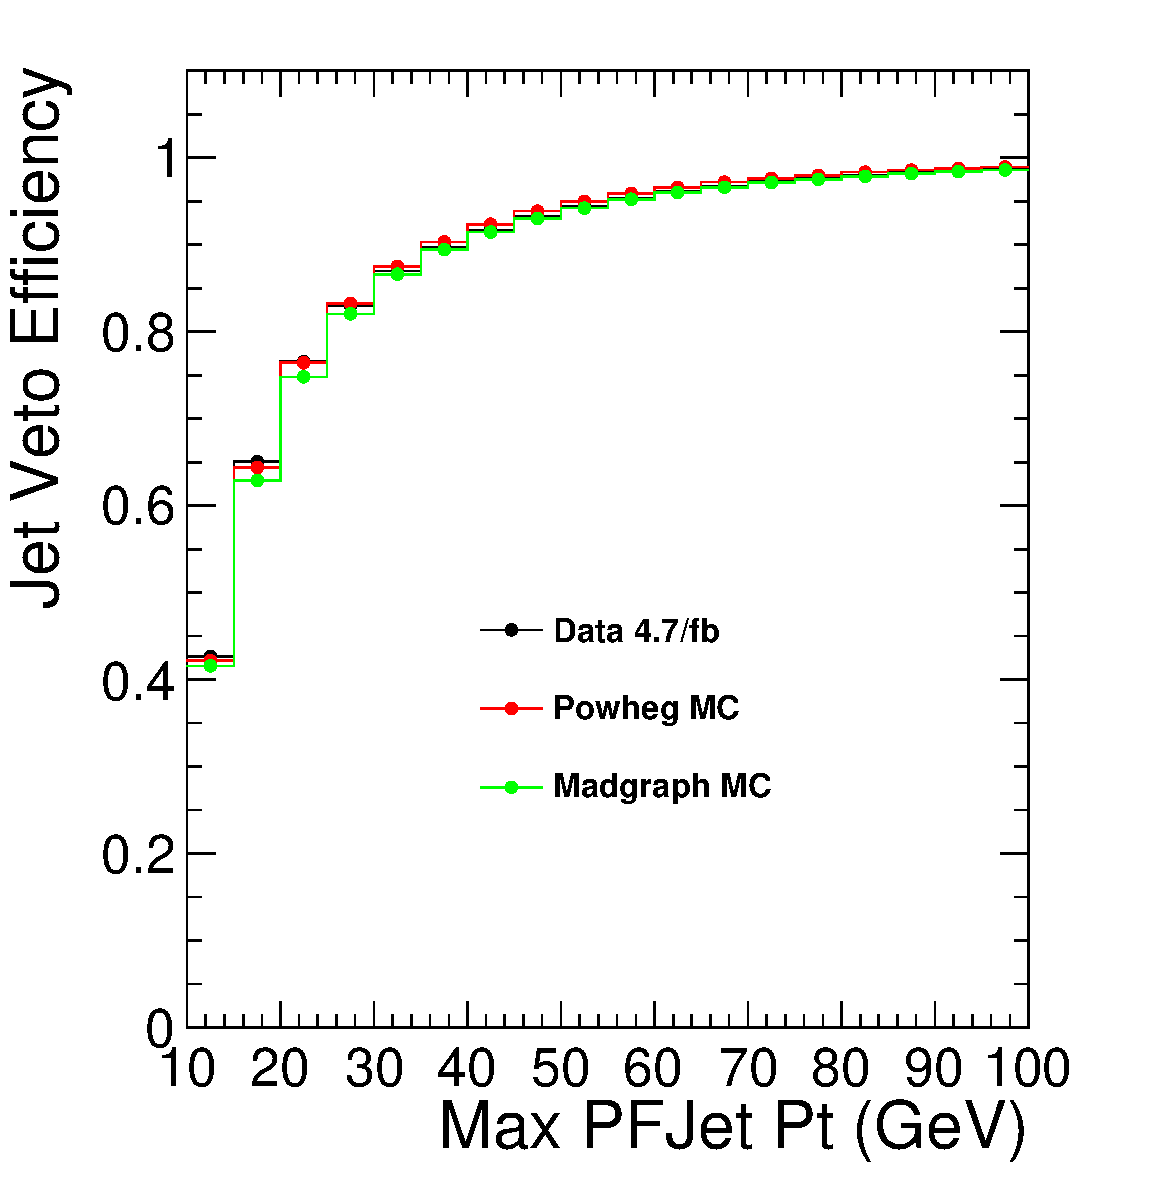
\includegraphics[width=0.49\textwidth]{figures/Zjetvetoeff_ee.pdf}
   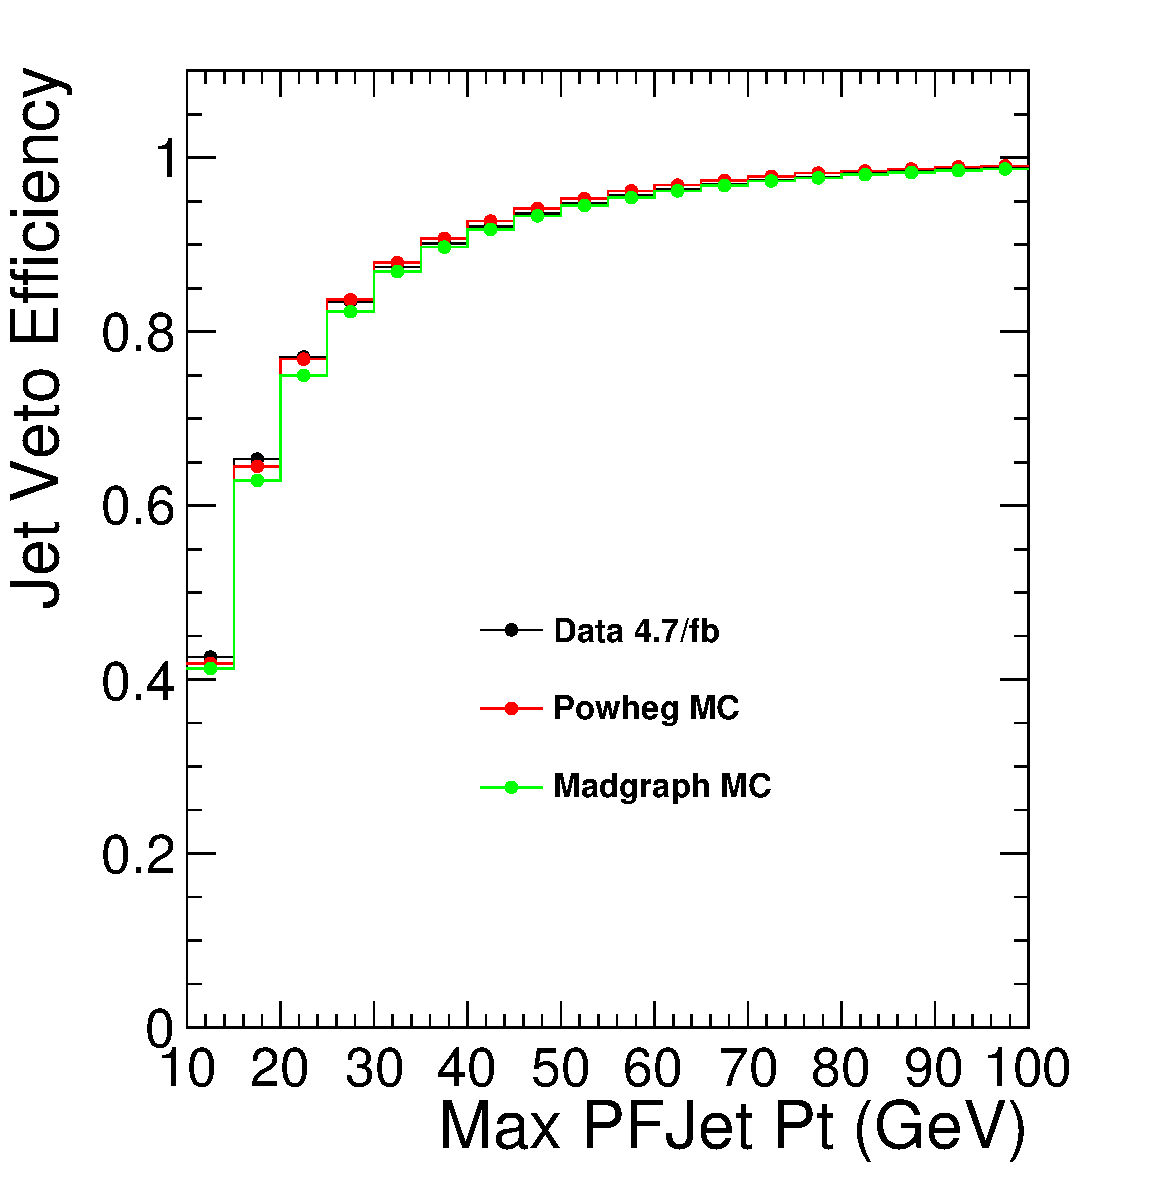
\includegraphics[width=0.49\textwidth]{figures/Zjetvetoeff_mm.pdf}
    \caption{Jet veto efficiency of $\dyee$ (left) and $\dymm$ (right) events, 
    comparing data with Powheg and Madgraph simulations.}
    \label{fig:zJetVetoEff}
  \end{center}
\end{figure}
%%%%%%%%%%%%%%%%%%%%%%%%%%%%%%


%The data to simulation correction factor is close to unity for the zero-jet and 1-jet bins, 
%while we observe some disagreement for events with at least two reconstructd jets. 
%This is not surprising since Powheg is an NLO generator, and 
%only expected to produce an accurate description for events 
%containing up to one jet. For instance, the comparison between data and Madgraph 
%simulation, which accounts for leading order diagrams containing up to four additional
%partons, gives much better agreement in the 2-jet bin. 

